\section{Challenges}

\begin{frame}{Challenges}

% \begin{itemize}

%     \item Performance relies heavily on the quality of prompts
%     \item Deploying LLMs for toxic content detection can incur both high run-time costs and high latency 
%     \item \textbf{Existing works}-Bootstrapping and Distilling LLM's
%     \begin{itemize}
%         \item Decision-Tree-of-Thought
%         \item Fine-tune a suitable student LM with a smaller model size
%     \end{itemize}
%     \begin{figure}
%         \centering
%         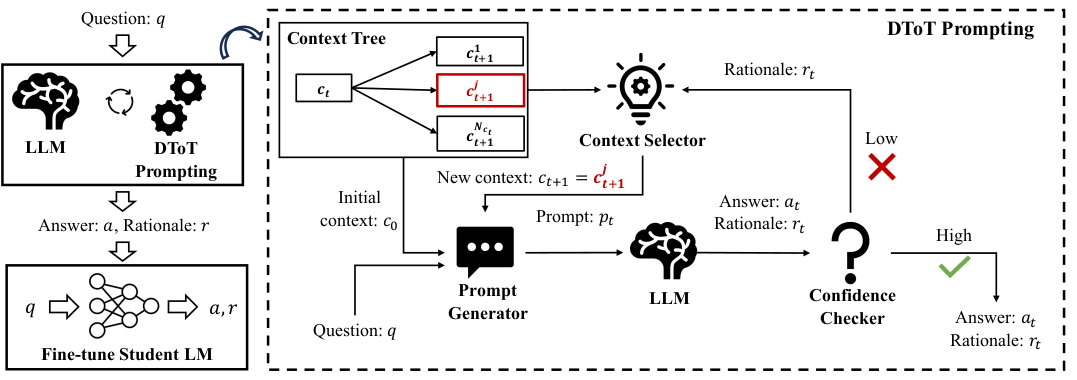
\includegraphics[width=1\linewidth]{images/BD_LLM.png}
%         \caption{Illustration of BD-LLM}
%         \label{fig:1}
%     \end{figure}

% \end{itemize}

\begin{itemize}

    \item A major challenge in detecting toxicity is that toxicity is relative.
    \item Some may think that some content is toxic, while others may not.
    \item This happens due to different perceptions of people.
    \item In addition, the datasets being used are also biased.
    \item For example:
    \begin{itemize}
        \item "I'm going to kill Amy" is labelled as not toxic in the DHate dataset, whereas it falls in the "Threatening" category.
        \item "A dude with money can only impress a broke bitch" is labelled as not toxic in the SBIC dataset, whereas many may think it is (due to vulgarity).
    \end{itemize}

\end{itemize}

\begin{itemize}
    \item 
\end{itemize}

\end{frame}
